\section{Sucção} % (fold)
\label{sec:sucção2}
	Essa seção visa documentar o método de construção do sistema de sucção do robô, descrevendo a construção dos protótipos e as decisões tomadas com base em testes realizados em cada protótipo. 

	\subsection{Metodologia de construção}
	\label{sub:metodologia_de_construção}
		Para a execução do projeto proposto foram adquiridos três coolers comerciais de 14 cm com as seguintes especificações.

		\begin{table}[H]
			\centering
			\caption{Dados do cooler}
			\label{tab:especificações_coolers}
			\begin{tabular}{ll}
				Potencia                                              & 1.44 W               \\
				Voltagem                                              & 12 V                 \\
				Velocidade                                            & 1200+-10\% RPM       \\
			\begin{tabular}[c]{@{}l@{}}Fluxo de ar\end{tabular} & 1.36 $m^3$/min (48 CFM)
			\end{tabular}
		\end{table}
		
		O projeto baseava-se em apenas dois coolers, mas foram adquiridos três caso o resultado com dois não retornasse uma boa sucção. A montagem deste primeiro protótipo consiste nos coolers ligados lado a lado dentro de uma caixa hermeticamente fechada. Foi feita a estrutura da caixa em papelão, seguindo a estrutura mostrada na figura \ref{img:vista_isometrica_de_montagem}. Com a caixa pronta e selada, foram feitos os furos para encaixar os coolers. Na parede oposta aos coolers foi feito um furo de pequeno diâmetro por onde entra o ar que deve ser sugado pelas hélices do cooler. 

		\begin{figure}[H]
			\centering
			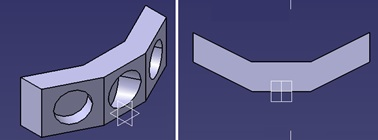
\includegraphics[scale=1]{figuras/asppc2_1.jpg}
			\caption{Vista isométrica e superior da montagem, onde os buracos representam a posição dos coolers.}
			\label{img:vista_isometrica_de_montagem}
		\end{figure}

		Para testar a funcionalidade de um novo modelo de construção a também da eficiência de apenas um cooler, foi feito um protótipo em menor escala utilizando um cooler menor de 5 cm e um compartimento de plástico de formato cilíndrico. Foi fixado o cooler no topo do cilindro e foi feito um furo de diâmetro menor abaixo dele. Foi feito um furo na lateral do cilindro para encaixar um tubo por onde o ar é sugado. O protótipo 2 é mostrado na figura \ref{img:cooler_5cm}.

		\begin{figure}[H]
			\centering
			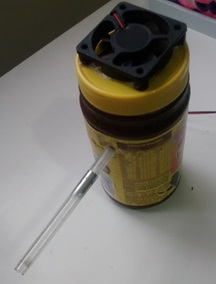
\includegraphics[scale=1]{figuras/asppc2_2.jpg}
			\caption{Montagem com cooler de 5 cm.}
			\label{img:cooler_5cm}
		\end{figure}

		Após a validação do protótipo 2, o mesmo modelo foi construído em maior escala utilizando o cooler maior a fim de verificar a funcionalidade dele. Utilizando um compartimento maior, desta vez de metal, e uma mangueira de maior diâmetro na entrada do ar. O protótipo 3 é mostrado na figura \ref{img:cooler_14cm}.

		\begin{figure}[H]
			\centering
			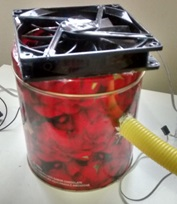
\includegraphics[scale=1]{figuras/asppc2_3.jpg}
			\caption{Montagem com cooler de 14 cm.}
			\label{img:cooler_14cm}
		\end{figure}

		O protótipo 3 foi construído para aumentar a potência do sistema construindo-o com dois coolers utilizando o mesmo esquema de construção. Também para reduzir a alimentação fornecida aos motores. Foi reduzida a altura do sistema, a fim de reduzir perdas de carga e adicionado um cooler em uma das paredes. Ao final obteve o seguinte protótipo:

		\begin{figure}[H]
			\centering
			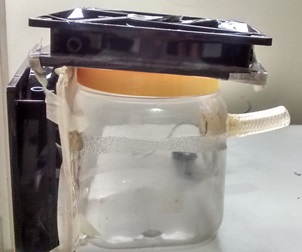
\includegraphics[scale=1]{figuras/asppc2_4.jpg}
			\caption{Protótipo com dois coolers de 14 cm.}
			\label{img:coolers_14cm}
		\end{figure}

		Para a tentativa de construção um novo tipo de protótipo, foram estudadas a opção de utilizar novas hélices. As hélices são um tipo de “ventilador axial”, que força o ar a passar por elas, gerando um fluxo de ar que segue transversal à direção do cooler. Existe também outro tipo de ventilador, conhecido como “ventilador centrífugo”, onde suas hélices são dispostas de forma diferente, mostradas na figura \ref{img:ventilador_centrífugo}.

		\begin{figure}[H]
			\centering
			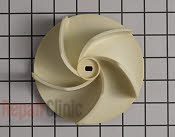
\includegraphics[scale=1]{figuras/asppc2_5.jpg}
			\caption{Hélices do ventilador centrífugo.}
			\label{img:ventilador_centrífugo}
		\end{figure}

		O “ventilador centrífugo” acelera o ar radialmente, fazendo com que a energia cinética da rotação das hélices aumente a pressão do ar, resultando em um fluxo de alta velocidade na saída. Foi escolhida essa hélice para a construção de novos protótipos.

		\begin{figure}[H]
			\centering
			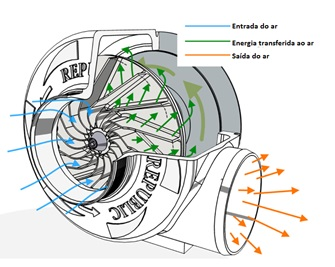
\includegraphics[scale=1]{figuras/asppc2_6.jpg}
			\caption{Fluxo de ar em um ventilador de ar centrífugo.\href{https://www.republic-mfg.com/blowers/republic-centrifugal-blower.asp}{Republic Manufacturing}}
			\label{img:fluxo_de_ar_ventilador_centrífugo}
		\end{figure}

		Para evitar o problema de falta de potência, foi escolhido um motor com maior potência e rotação nominal se comparado ao motor do cooler. Foi escolhido um motor DC 12V com as especificações apresentadas na tabela \ref{tab:motor_12V}.

		\begin{table}[H]
			\centering
			\caption{Dados do motor DC 12 Volts.}
			\label{tab:motor_12V}
			\begin{tabular}{ll}
				Potencia   & 40.55W          \\
				Voltagem   & 13.5 V          \\
				Velocidade & 28086+-10\% RPM \\
				Torque     & 55.19 mN.m     
			\end{tabular}
		\end{table}

		As hélices foram construídas em alumínio. Todas foram cortadas com o mesmo tamanho e levemente curvadas. Para encaixá-las no eixo do motor foi feito uma pequena base de formato hexagonal também em alumínio com um furo no centro do tamanho do eixo do motor. As hélices foram coladas na base com epóxi.

		\begin{figure}[H]
			\centering
			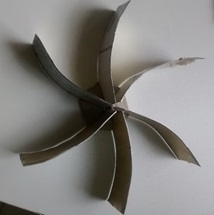
\includegraphics[scale=1]{figuras/asppc2_7.jpg}
			\caption{Hélices construídas em alumínio.}
			\label{img:hélices_alumínio}
		\end{figure}

		Seguindo o modelo da figura \ref{img:fluxo_de_ar_ventilador_centrífugo}, foi construída a estrutura para encaixar a hélice construída. Utilizando CD’s, papelão, plástico em formato cilíndrico a estrutura final do protótipo 5 é mostrada na figura \ref{img:protótipo_CD}: 

		\begin{figure}[H]
			\centering
			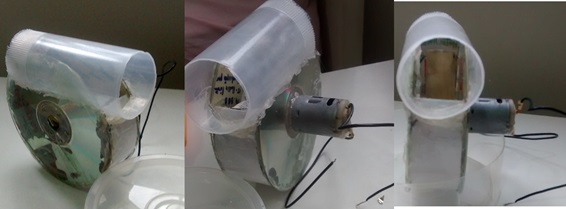
\includegraphics[scale=1]{figuras/asppc2_8.jpg}
			\caption{Vistas do protótipo feito com CD’s.}
			\label{img:protótipo_CD}
		\end{figure}

		Para aprimorar a construção utilizando esse tipo de hélice, foi construído um protótipo final utilizando uma hélice comercial e motor com as seguintes especificações:

		\begin{table}[]
			\centering
			\caption{Especificações do Motor}
			\label{tab:specsmotor}
			\begin{tabular}{ll}
				Potencia   & 52.8 W          \\
				Voltagem   & 12 V          \\
				Corrente     & 4.4 A     
			\end{tabular}
		\end{table}

		\begin{figure}[H]
			\centering
			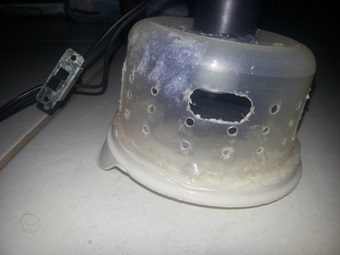
\includegraphics[scale=1]{figuras/asppc2_9.jpg}
			\caption{Motor de 52.8W instalado na estrutura de aspiração.}
			\label{img:estrutura_motor_52.8W}
		\end{figure}

		Foi realizada a montagem do protótipo utilizando a nova hélice. Foram utilizados dois compartimentos de plásticos, em um foi acoplado o conjunto hélice motor, como mostra a figura \ref{img:estrutura_motor_52.8W}. Nas laterais foram feitos furos para a saída de ar. Foi colocada uma divisão entre os dois compartimentos com um filtro para a sujeira. Foi feito um furo no segundo compartimento para encaixar a mangueira a qual irá ser a ponta da sucção.

		\begin{figure}[H]
			\centering
			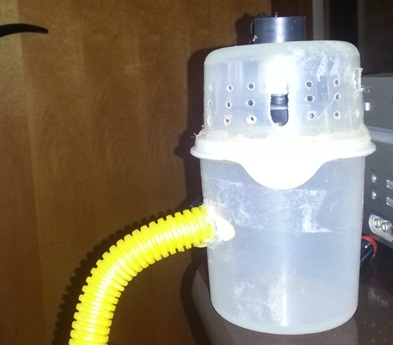
\includegraphics[scale=1]{figuras/asppc2_10.jpg}
			\caption{Sistema de sucção com o compartimento de sujeira.}
			\label{img:sistema_com_compartimento}
		\end{figure}

		Para aumentar a eficiência de limpeza, foi adicionado ao sistema de sucção uma vassoura mágica. A fricção dela com o solo faz com que a sujeira seja carregada para seu compartimento interno, mas para garantir uma boa limpeza ela deve passar pelo mesmo local várias vezes. Como o robô irá percorrer a trajetória em linha reta com velocidade constante sem realizar muitas passagens pelo mesmo local, foi acoplado um motor DC de 6V e 0.1 A no eixo da vassoura para garantir um aumento na eficiência na coleta da sujeira. 

		\begin{figure}[H]
			\centering
			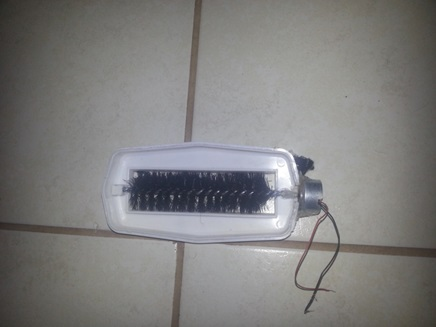
\includegraphics[scale=1]{figuras/asppc2_11.jpg}
			\caption{Escova mágica conectada ao motor DC de 6V.}
			\label{img:escova_com_motor}
		\end{figure}

		Foi feita a conexão entre eles por uma mangueira sanfonada, para que ela sugue as partículas de sujeiras que a vassoura colhe. Foi feito um furo na parte superior da estrutura da vassoura da forma da ponta de mangueira, que foi achatada para aumentar o comprimento de aspiração da sujeira que fica interna a vassoura mágica. O resultado do protótipo final é mostrado na figura \ref{img:sistema_completo}.

		\begin{figure}[H]
			\centering
			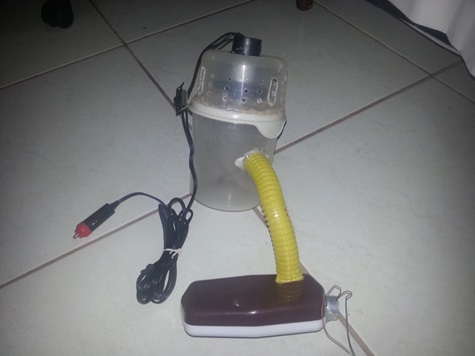
\includegraphics[scale=1]{figuras/asppc2_13.jpg}
			\caption{Subsistema de sucção completo.}
			\label{img:sistema_completo}
		\end{figure}

		Foi realizado o teste das duas peças integradas, simulou-se o movimento do robô passando-o apenas uma vez por cima da sujeira. O resultado foi positivo, o sistema foi capaz de colher cerca de 80\% das partículas que foram colocadas para teste.
	% subsection metodologia de construção (end)
% section sucção (end)

\subsection{Validação experimental} % (fold)
	\label{sub:validação_experimental}

\subsubsection{Protótipo 1}
Após a finalização da construção do protótipo 1, os coolers foram ligados à voltagem de 12V com corrente de 1.5 A. O resultado não foi satisfatório. Não houve nenhuma sucção mesmo alterando o diâmetro do buraco por onde entra o ar e sua posição. Foi suposto que o problema seriam os coolers. Então foi planejada uma montagem utilizando apenas um deles para verificar seu funcionamento isolado, para isso foi construído o protótipo 3. 

\subsubsection{Protótipo 2}
Antes de realizar testes com o protótipo 3, foi realizado o teste do protótipo 2 a fim de testar o funcionamento do novo modelo de construção, Foi ligado na fonte a 12 V. O teste apresentou resultados positivos, apesar da sucção fraca por conta da voltagem e corrente do cooler serem baixos. De posse dos bons resultados com o modelo, seguiu-se a construção e testes do protótipo 3

\subsubsection{Protótipo 3}
Foi fornecido a tensão de 12V e corrente de 1.5 A ao cooler do protótipo 3. O resultado foi negativo, pois apresentou uma eficiência muito baixa, com sucção quase imperceptível. Utilizando uma fonte de tensão, foi-se elevando a tensão até que ele indicasse uma melhora. Foi observado que enquanto a tensão era modificada, as hélices passavam a girar com maior velocidade e consequentemente sugavam com maior força. Ao fornecer o valor de tensão de 30 V, foi que o sistema alcançou um resultado que seria ótimo para o projeto. Mas seria inviável a fabricação do robô com uma bateria que fornecesse tal tensão.

\subsubsection{Protótipo 4}    
O último teste utilizando estes coolers consistiu em ligá-los a 12 V e 1 A cada. Era esperado que com essa nova montagem a eficiência fosse aumentada, pois a potência do sistema foi dobrada. Mas o resultado foi negativo, pois não apresentou mudanças com relação ao modelo utilizando apenas um cooler. Com base nos resultados obtidos com os protótipos mostrados, o grupo chegou à conclusão de que os coolers não seriam utilizados, pois não mostraram resultados bons que fossem viáveis ao projeto. Os motores elétricos dos coolers possuíam uma potência incompatível com o tipo e o tamanho da hélice do mesmo, gerando um fluxo de massa baixo, menor que o indicado pelos fabricantes. 

\subsubsection{Protótipo 5}
Foi realizado o teste com o protótipo utilizando a hélice que foi construída. Mas por defeitos de fabricação, as hélices durante a rotação colidiam com a estrutura, assim o ar era soprado com menor velocidade, consequentemente sugava um fluxo baixo de ar. 
Foi feita outro protótipo utilizando o mesmo modelo de hélice construída com CD seguindo o mesmo modelo de estrutura, mas novamente, as hélices não giravam livremente, pois colidiam com as outras partes da estrutura. Graças à essas assimetrias e defeitos de fabricação foi observado uma grande vibração do sistema. Diante da dificuldade de construir uma estrutura sem defeitos e visando reduzir as vibrações, para que ela não danifique a estrutura do robô e aumentar a eficiência do ventilador, foi construído o protótipo 6.

\subsubsection{Protótipo 6}
Os testes com esse protótipo foi feito ligando-a fonte de 12V e 4.4 A. O resultado foi positivo apresentando uma sucção forte, sugando toda a sujeira que foi disponibilizada para o teste. O teste com a vassoura mágica também foi realizado, ligando o motor do eixo à fonte. Observou-se que por conta da grande velocidade de rotação do motor, as partículas de sujeiras eram lançadas para longe, ao invés de serem carregadas para seu interior. Foi colocado um tecido com pelos atrás da vassoura, limitando o movimento de partículas naquela direção, garantindo que elas fossem depositadas no interior da vassoura. Com esses dois subsistemas de limpeza prontos e funcionando, foi feita a conexão entre eles e realizado o teste. Os dois motores foram ligados à tensão de 12V e 6V e simulou-se o movimento do robô passando-o apenas uma vez por cima da sujeira. O resultado foi positivo, o sistema foi capaz de colher cerca de 60\% das partículas que foram colocadas para teste.
